\documentclass[UTF8]{ctexart}

\usepackage{indentfirst}
\usepackage{caption}
\usepackage{graphicx}
\usepackage{listings}
\usepackage{xcolor}


\lstset{language=C}
\lstset{language=Python}
\lstset{breaklines}
\lstset{extendedchars=false}
\lstset{numbers=left,
frame = single,
title = \lstname} 

\usepackage{algorithm}
\usepackage{algorithmic}
\usepackage{float}


\renewcommand{\baselinestretch}{1.5}

\setlength{\parindent}{2em}

\title{操作系统第一组实验报告}
\author{漆耘含\\2016011058}
\date{}

\begin{document}
\maketitle
\section{银行柜员服务问题}
\subsection{问题描述}
银行有n个柜员负责为顾客服务,顾客进入银行先取一个号码,然后等着叫号。当某个柜员空闲下来,就叫下一个号。\par
编程实现该问题,用P、V操作实现柜员和顾客的同步。\par

\subsection{实现要求}
1. 某个号码只能由一名顾客取得;\par
2. 不能有多于一个柜员叫同一个号;\par
3. 有顾客的时候,柜员才叫号;\par
4. 无柜员空闲的时候,顾客需要等待\par
5. 无顾客的时候,柜员需要等待。\par
\subsection{实现提示}
1. 互斥对象:顾客拿号,柜员叫号;\par
2. 同步对象:顾客和柜员;\par
3. 等待同步对象的队列:等待的顾客,等待的柜员;\par
4. 所有数据结构在访问时也需要互斥。\par
\subsection{测试文本格式}
测试文件由若干记录组成,记录的字段用空格分开。记录第一个字段是顾客序号,第二字段为顾客进入银行的时间,第三字段是顾客需要服务的时间。\par
下面是一个测试数据文件的例子:\par
\qquad 1 1 10\par
\qquad 2 5 2\par
\qquad 3 6 3\par
\subsection{输出要求}
对于每个顾客需输出进入银行的时间、开始服务的时间、离开银行的时间和服务柜员号。\par

\section{实验环境}
Ubuntu\quad 18.04.1 \quad LTS, 64位操作系统\par
具体配置如下:\par
\begin{figure}[!h]
\centering
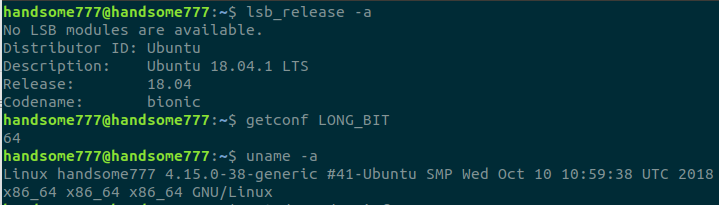
\includegraphics[scale = 0.7,bb=0 0 518 148]{ubuntu_info.png}
\label{img1}
\end{figure}

\section{原理分析}
针对这个银行柜台这个问题,先分清有两个对象,一个是柜台(Counter),另一个是消费者(Customer)。下面就分别对柜台线程和消费者线程进行解析。\par
\subsection{柜台}
每一个柜台之间是相互独立的,所以刚开始应该为每一个柜台创建一个进程,以保证独立性。同时,柜台还需要编号、锁变量、进程变量等,因此柜台被封装为一个结构体,结构体的设计如下:\par
\begin{algorithm}
\caption{struct Counter}
$pthread\_ t$ $ c\_ pthread_t$;//pthread var\\
$pthread\_ mutex\_ t$ $ c\_ mutex\_ t$;//mutex var\\
$pthread\_ cond\_ t$ $ c\_ cond\_ t$;//cond var\\
\end{algorithm}


在柜台和消费者之外,有一个队列(queue),里面是消费者按时间进入的顺序,先进先出,后进后出。在柜台流程刚开始的时候,先判断取出一个资源后,信号量是否小于等于0,如果小于等于0,则陷入阻塞,直到有消费者进入增加资源唤醒柜台,这时柜台进程才继续运行。\par
因为柜台进程之间是相互独立的,但他们都是从同一个队列(queue)里面读取消费者,
因此可能被同时取出去,所以要加一个判断,即取出的消费者是否有对应的柜台号(消费者结构体定义见下一个小节),如果有,则继续取或者阻塞,如果没有,则柜台与消费者匹配成功,然后进入服务,在这个时候要及时修改消费者的对应柜台编号,避免被同时服务的可能,柜台会陷入等待状态($pthread\_ cond\_ wait$),直到消费者服务完成(sleep),发送一个signal信号,唤醒柜台,然后结束服务。\par
值得注意的是,在所有消费者完成服务之后,所有的柜台进程都会陷入阻塞中,程序无法正常执行,因此需要设立一个全局变量($finish\_ cus \_ num$),在主函数中会陷入忙等状态($pthread\_ cond\_ wait$),在每次柜台服务完一个消费者之后,$finish\_ cus\_ num++$,并发送一个signal,唤醒主程序中的忙等,当$finish\_ cus \_ num$等于消费者总数的时候,跳出while循环,程序结束。\par

\subsection{消费者}
每一个消费者之间是相互独立的,需要为每一个消费者创建一个进程。消费者的结构体定义如下:\par
\begin{algorithm}
\caption{struct Customer}
$pthread\_ t$ $ cus\_ pthread\_ t$;//pthread var\par
$pthread\_ mutex\ _t $ $cus\_ mutex\_ t$;//mutex var\par
$pthread\_ cond\_ t$ $ cus\_ cond\_ t$;//cond var\par
int $cus\_ id$;//customer id\par
int $coun\_ id$;//counter id\par
int $enter\_ time$;//enter time\par
int $wait\_ time$;//serve time\par
\end{algorithm}

消费者的信息是从文件中读取进来的,因此为了实现模拟消费者在不同时刻进来的情形,需要在进程刚开始的时候sleep一段时间(各个消费者是不相同的),在sleep一段时间后,按时间(执行)的顺序依次进入队列,以便后续过程。消费者在没有柜台服务的时候,是需要等到的,即用一个while循环,判断条件是该消费者的服务柜台号不为-1(初始值为-1,代表没有柜台服务),当柜台和消费者匹配之后,由柜台修改消费者的柜台号,修改之后,消费者跳出循环,进入接受服务阶段,即sleep(服务)一段时间之后,发送一个signal给柜台,唤醒柜台,即表示服务已经结束。\par

\subsection{程序流程}
首先从$customer\_ data.dat$里面读取用户信息并保存在customer结构体数组中,然后进行初始化,为每一个柜台和每一个消费者进行初始化(创建进程、锁变量初始化),然后消费者进行入队列(queue),开始上述两小节所描述的流程\par

\begin{algorithm}
\caption{bank counter-customer algorithm}
\begin{algorithmic}[1]
\STATE algorithm describtion\par
\STATE	\qquad load data from "$customer\_ data.dat$";\par
\STATE	\qquad initial varibales($pthread\_ mutex_t,pthread\_ cond_t$);	\par
\STATE	\qquad create counter thread;	\par
\STATE	\qquad create customer thread;	\par
\STATE \qquad for each counter \par
\STATE	\qquad\qquad record it's id;\par
\STATE	\qquad\qquad if (num of customer $<=$ 0)\par
\STATE	\qquad\qquad\qquad stuck until num of customer $>$ 0;\par
\STATE	\qquad\qquad else\par
\STATE	\qquad\qquad\qquad arouse a customer;\par 
\STATE	\qquad\qquad\qquad customer receive serve from that counter; \par
\STATE	\qquad\qquad wait and serve next customer;\par
\STATE	\qquad for each customer:\par
\STATE	\qquad\qquad come into bank in time order(after create, sleep for a while);\par
\STATE	\qquad\qquad wait until a counter arouse it;\par
\STATE	\qquad\qquad begin serve\par
\STATE	\qquad\qquad after serve, leave bank;\par
\STATE	\qquad when all customers are served, then program finfish;	\par
\end{algorithmic}
\end{algorithm}


\section{运行结果及分析}
\subsection{生成测试样本}
为了检验程序的正确性,我编写了一个生成随机样本的python程序,用来生成指定数目的顾客。(具体代码见附录),下面展示随机生成的样本(一部分):\par
3 1 1\par
1 1 5\par
2 2 5\par
3 2 8\par
4 3 5\par
5 5 10\par
6 8 5\par
7 8 9\par
8 9 6\par
9 9 1\par
10 10 3\par
11 11 2\par
12 14 6\par
13 15 9\par

\section{程序运行结果}
生成100个顾客,柜台数为5的运行结果:\\
customer id:0, enter at 1, served at 1, leave at 2,served by counter id:1
\\
customer id:1, enter at 1, served at 1, leave at 6,served by counter id:0
\\
customer id:2, enter at 2, served at 2, leave at 7,served by counter id:2
\\
customer id:4, enter at 3, served at 3, leave at 8,served by counter id:4
\\
customer id:3, enter at 2, served at 2, leave at 10,served by counter id:3
\\
customer id:9, enter at 9, served at 10, leave at 11,served by counter id:3
\\
customer id:6, enter at 8, served at 8, leave at 13,served by counter id:0
\\
customer id:10, enter at 10, served at 11, leave at 14,served by counter id:3
\\
customer id:5, enter at 5, served at 5, leave at 15,served by counter id:1
\\
customer id:8, enter at 9, served at 9, leave at 15,served by counter id:4
\\
customer id:11, enter at 11, served at 13, leave at 15,served by counter id:0
\\
customer id:7, enter at 8, served at 8, leave at 17,served by counter id:2
\\
customer id:14, enter at 15, served at 15, leave at 19,served by counter id:4
\\
customer id:12, enter at 14, served at 14, leave at 20,served by counter id:3
\\
customer id:13, enter at 15, served at 15, leave at 24,served by counter id:1
\\
customer id:15, enter at 16, served at 17, leave at 26,served by counter id:0
\\
customer id:20, enter at 21, served at 26, leave at 28,served by counter id:0
\\
customer id:18, enter at 20, served at 21, leave at 28,served by counter id:4
\\
customer id:16, enter at 19, served at 19, leave at 28,served by counter id:2
\\
customer id:21, enter at 21, served at 28, leave at 30,served by counter id:0
\\
customer id:17, enter at 20, served at 21, leave at 31,served by counter id:3
\\
customer id:24, enter at 24, served at 30, leave at 32,served by counter id:0
\\
customer id:23, enter at 22, served at 29, leave at 34,served by counter id:2
\\
customer id:19, enter at 21, served at 24, leave at 34,served by counter id:1
\\
customer id:25, enter at 28, served at 31, leave at 35,served by counter id:3
\\
customer id:26, enter at 28, served at 32, leave at 35,served by counter id:0
\\
customer id:22, enter at 22, served at 28, leave at 37,served by counter id:4
\\
customer id:29, enter at 31, served at 35, leave at 37,served by counter id:3
\\
customer id:30, enter at 32, served at 36, leave at 39,served by counter id:0
\\
customer id:28, enter at 31, served at 35, leave at 39,served by counter id:1
\\
customer id:27, enter at 29, served at 34, leave at 40,served by counter id:2
\\
customer id:31, enter at 33, served at 37, leave at 43,served by counter id:4
\\
customer id:36, enter at 34, served at 40, leave at 43,served by counter id:2
\\
customer id:35, enter at 34, served at 39, leave at 44,served by counter id:0
\\
customer id:33, enter at 34, served at 39, leave at 44,served by counter id:1
\\
customer id:32, enter at 33, served at 37, leave at 45,served by counter id:3
\\
customer id:34, enter at 34, served at 43, leave at 45,served by counter id:4
\\
customer id:37, enter at 35, served at 43, leave at 47,served by counter id:2
\\
customer id:40, enter at 39, served at 45, leave at 49,served by counter id:3
\\
customer id:43, enter at 42, served at 50, leave at 52,served by counter id:3
\\
customer id:38, enter at 35, served at 44, leave at 53,served by counter id:0
\\
customer id:39, enter at 36, served at 44, leave at 54,served by counter id:1
\\
customer id:42, enter at 40, served at 48, leave at 55,served by counter id:2
\\
customer id:41, enter at 39, served at 46, leave at 55,served by counter id:4
\\
customer id:48, enter at 46, served at 55, leave at 61,served by counter id:4
\\
customer id:46, enter at 44, served at 54, leave at 61,served by counter id:1
\\
customer id:44, enter at 43, served at 52, leave at 62,served by counter id:3
\\
customer id:45, enter at 43, served at 53, leave at 63,served by counter id:0
\\
customer id:47, enter at 46, served at 55, leave at 65,served by counter id:2
\\
customer id:49, enter at 47, served at 61, leave at 65,served by counter id:4
\\
customer id:51, enter at 50, served at 62, leave at 66,served by counter id:3
\\
customer id:50, enter at 48, served at 61, leave at 66,served by counter id:1
\\
customer id:54, enter at 53, served at 65, leave at 67,served by counter id:4
\\
customer id:56, enter at 54, served at 68, leave at 71,served by counter id:4
\\
customer id:57, enter at 54, served at 67, leave at 72,served by counter id:1
\\
customer id:59, enter at 59, served at 72, leave at 73,served by counter id:1
\\
customer id:58, enter at 56, served at 71, leave at 73,served by counter id:4
\\
customer id:52, enter at 50, served at 64, leave at 74,served by counter id:0
\\
customer id:53, enter at 51, served at 65, leave at 74,served by counter id:2
\\
customer id:55, enter at 54, served at 66, leave at 74,served by counter id:3
\\
customer id:63, enter at 64, served at 74, leave at 76,served by counter id:2
\\
customer id:62, enter at 63, served at 74, leave at 79,served by counter id:0
\\
customer id:60, enter at 62, served at 73, leave at 82,served by counter id:1
\\
customer id:61, enter at 62, served at 73, leave at 82,served by counter id:4
\\
customer id:66, enter at 65, served at 79, leave at 83,served by counter id:0
\\
customer id:67, enter at 70, served at 82, leave at 84,served by counter id:1
\\
customer id:65, enter at 65, served at 77, leave at 85,served by counter id:2
\\
customer id:64, enter at 64, served at 75, leave at 85,served by counter id:3
\\
customer id:68, enter at 70, served at 83, leave at 86,served by counter id:4
\\
customer id:70, enter at 71, served at 85, leave at 88,served by counter id:1
\\
customer id:72, enter at 72, served at 85, leave at 90,served by counter id:3
\\
customer id:74, enter at 72, served at 88, leave at 91,served by counter id:1
\\
customer id:77, enter at 74, served at 91, leave at 93,served by counter id:1
\\
customer id:69, enter at 71, served at 83, leave at 93,served by counter id:0
\\
customer id:75, enter at 73, served at 90, leave at 94,served by counter id:3
\\
customer id:71, enter at 71, served at 85, leave at 95,served by counter id:2
\\
customer id:76, enter at 74, served at 93, leave at 95,served by counter id:1
\\
customer id:73, enter at 72, served at 86, leave at 96,served by counter id:4
\\
customer id:79, enter at 76, served at 94, leave at 98,served by counter id:3
\\
customer id:81, enter at 80, served at 96, leave at 101,served by counter id:1
\\
customer id:84, enter at 81, served at 101, leave at 102,served by counter id:1
\\
customer id:82, enter at 80, served at 96, leave at 102,served by counter id:4
\\
customer id:78, enter at 76, served at 93, leave at 102,served by counter id:0
\\
customer id:86, enter at 82, served at 102, leave at 104,served by counter id:4
\\
customer id:80, enter at 79, served at 95, leave at 105,served by counter id:2
\\
customer id:87, enter at 83, served at 103, leave at 108,served by counter id:0
\\
customer id:83, enter at 81, served at 99, leave at 108,served by counter id:3
\\
customer id:85, enter at 82, served at 102, leave at 108,served by counter id:1
\\
customer id:89, enter at 84, served at 105, leave at 109,served by counter id:2
\\
customer id:88, enter at 83, served at 104, leave at 111,served by counter id:4
\\
customer id:96, enter at 91, served at 112, leave at 113,served by counter id:4
\\
customer id:90, enter at 86, served at 108, leave at 115,served by counter id:0
\\
customer id:91, enter at 88, served at 108, leave at 115,served by counter id:3
\\
customer id:93, enter at 89, served at 108, leave at 115,served by counter id:1
\\
customer id:92, enter at 89, served at 110, leave at 117,served by counter id:2
\\
customer id:95, enter at 91, served at 115, leave at 120,served by counter id:0
\\
customer id:94, enter at 91, served at 113, leave at 121,served by counter id:4
\\
customer id:99, enter at 95, served at 117, leave at 122,served by counter id:2
\\
customer id:97, enter at 92, served at 115, leave at 122,served by counter id:3
\\
customer id:98, enter at 92, served at 115, leave at 124,served by counter id:1
\\

结果分析:\par
从上面的运行结果来看,比如对于柜台1,先服务顾客0并于时刻2结束服务,然后在时刻5服务顾客5并于时刻15结束,再在时刻15服务顾客13并于时刻24结束,依次类推,对每一个柜台都是这样的,运行结果没问题。\par

\section{思考题}

\subsection{柜员人数和顾客人数对结果分别有什么影响}
顾客人数很多,而柜台人数很少的时候,最后一名顾客结束服务的时刻,和柜台数量大致程反比。当柜台数较少,同一时间能服务的的顾客数就越少,吞吐量越小,顾客等待的时间也就越长。\par
当柜台数较多时,同一时间能服务的顾客就越多,系统的吞吐量就越大,顾客等待时间就越短。\par

\subsection{实现互斥的方法有哪些?各自有什么特点?效率如何?}
实现互斥的方法有:禁止中断、自旋锁、互斥锁、信号量\par
禁止中断:在内核态小代码段使用,用户态没有这样的接口,效率高;\par
自旋锁:忙等待,特点是死循环占满CPU,效率低;\par
互斥锁:用阻塞,不会浪费CPU资源,效率高;\par
信号量:可以实现多个生产、消费的互斥,有P、V两种操作,效率高;\par

\section{实验总结}
为了完成这次实验,我翻看了一些linux多线程编程的参考书,查阅了很多资料,这让我对linux更加熟悉,同时对线程进程的理解更加深刻。\par
虽然这次实验的难度并不是很大,但它带给了我全新的体验,因为之前从来没进行过多线程的编程,调试起来觉得特别困难,所以这对我来说是一个比较大的挑战,后来我分段输出,根据输出结果来分析,最终成功完成实验。

\section{其他}
\subsection{运行代码指令}
1. gcc -o test test.c -lpthread\par
2. ./test
\subsection{附录}
附录1:test.c(算法代码)\par
附录2:$gen\_ data.py$(生成用户数据代码)\par

\newpage
附录1:主程序(test.c)\par
\lstinputlisting{test.c}

\newpage
附录2:生成用户数据程序(datagen.py)\par
\lstinputlisting{datagen.py}




\end{document}